% Options for packages loaded elsewhere
\PassOptionsToPackage{unicode}{hyperref}
\PassOptionsToPackage{hyphens}{url}
%
\documentclass[
  ignorenonframetext,
]{beamer}
\usepackage{pgfpages}
\setbeamertemplate{caption}[numbered]
\setbeamertemplate{caption label separator}{: }
\setbeamercolor{caption name}{fg=normal text.fg}
\beamertemplatenavigationsymbolsempty
% Prevent slide breaks in the middle of a paragraph
\widowpenalties 1 10000
\raggedbottom
\setbeamertemplate{part page}{
  \centering
  \begin{beamercolorbox}[sep=16pt,center]{part title}
    \usebeamerfont{part title}\insertpart\par
  \end{beamercolorbox}
}
\setbeamertemplate{section page}{
  \centering
  \begin{beamercolorbox}[sep=12pt,center]{part title}
    \usebeamerfont{section title}\insertsection\par
  \end{beamercolorbox}
}
\setbeamertemplate{subsection page}{
  \centering
  \begin{beamercolorbox}[sep=8pt,center]{part title}
    \usebeamerfont{subsection title}\insertsubsection\par
  \end{beamercolorbox}
}
\AtBeginPart{
  \frame{\partpage}
}
\AtBeginSection{
  \ifbibliography
  \else
    \frame{\sectionpage}
  \fi
}
\AtBeginSubsection{
  \frame{\subsectionpage}
}
\usepackage{amsmath,amssymb}
\usepackage{iftex}
\ifPDFTeX
  \usepackage[T1]{fontenc}
  \usepackage[utf8]{inputenc}
  \usepackage{textcomp} % provide euro and other symbols
\else % if luatex or xetex
  \usepackage{unicode-math} % this also loads fontspec
  \defaultfontfeatures{Scale=MatchLowercase}
  \defaultfontfeatures[\rmfamily]{Ligatures=TeX,Scale=1}
\fi
\usepackage{lmodern}
\usetheme[]{Boadilla}
\ifPDFTeX\else
  % xetex/luatex font selection
\fi
% Use upquote if available, for straight quotes in verbatim environments
\IfFileExists{upquote.sty}{\usepackage{upquote}}{}
\IfFileExists{microtype.sty}{% use microtype if available
  \usepackage[]{microtype}
  \UseMicrotypeSet[protrusion]{basicmath} % disable protrusion for tt fonts
}{}
\makeatletter
\@ifundefined{KOMAClassName}{% if non-KOMA class
  \IfFileExists{parskip.sty}{%
    \usepackage{parskip}
  }{% else
    \setlength{\parindent}{0pt}
    \setlength{\parskip}{6pt plus 2pt minus 1pt}}
}{% if KOMA class
  \KOMAoptions{parskip=half}}
\makeatother
\usepackage{xcolor}
\newif\ifbibliography
\usepackage{color}
\usepackage{fancyvrb}
\newcommand{\VerbBar}{|}
\newcommand{\VERB}{\Verb[commandchars=\\\{\}]}
\DefineVerbatimEnvironment{Highlighting}{Verbatim}{commandchars=\\\{\}}
% Add ',fontsize=\small' for more characters per line
\usepackage{framed}
\definecolor{shadecolor}{RGB}{248,248,248}
\newenvironment{Shaded}{\begin{snugshade}}{\end{snugshade}}
\newcommand{\AlertTok}[1]{\textcolor[rgb]{0.94,0.16,0.16}{#1}}
\newcommand{\AnnotationTok}[1]{\textcolor[rgb]{0.56,0.35,0.01}{\textbf{\textit{#1}}}}
\newcommand{\AttributeTok}[1]{\textcolor[rgb]{0.13,0.29,0.53}{#1}}
\newcommand{\BaseNTok}[1]{\textcolor[rgb]{0.00,0.00,0.81}{#1}}
\newcommand{\BuiltInTok}[1]{#1}
\newcommand{\CharTok}[1]{\textcolor[rgb]{0.31,0.60,0.02}{#1}}
\newcommand{\CommentTok}[1]{\textcolor[rgb]{0.56,0.35,0.01}{\textit{#1}}}
\newcommand{\CommentVarTok}[1]{\textcolor[rgb]{0.56,0.35,0.01}{\textbf{\textit{#1}}}}
\newcommand{\ConstantTok}[1]{\textcolor[rgb]{0.56,0.35,0.01}{#1}}
\newcommand{\ControlFlowTok}[1]{\textcolor[rgb]{0.13,0.29,0.53}{\textbf{#1}}}
\newcommand{\DataTypeTok}[1]{\textcolor[rgb]{0.13,0.29,0.53}{#1}}
\newcommand{\DecValTok}[1]{\textcolor[rgb]{0.00,0.00,0.81}{#1}}
\newcommand{\DocumentationTok}[1]{\textcolor[rgb]{0.56,0.35,0.01}{\textbf{\textit{#1}}}}
\newcommand{\ErrorTok}[1]{\textcolor[rgb]{0.64,0.00,0.00}{\textbf{#1}}}
\newcommand{\ExtensionTok}[1]{#1}
\newcommand{\FloatTok}[1]{\textcolor[rgb]{0.00,0.00,0.81}{#1}}
\newcommand{\FunctionTok}[1]{\textcolor[rgb]{0.13,0.29,0.53}{\textbf{#1}}}
\newcommand{\ImportTok}[1]{#1}
\newcommand{\InformationTok}[1]{\textcolor[rgb]{0.56,0.35,0.01}{\textbf{\textit{#1}}}}
\newcommand{\KeywordTok}[1]{\textcolor[rgb]{0.13,0.29,0.53}{\textbf{#1}}}
\newcommand{\NormalTok}[1]{#1}
\newcommand{\OperatorTok}[1]{\textcolor[rgb]{0.81,0.36,0.00}{\textbf{#1}}}
\newcommand{\OtherTok}[1]{\textcolor[rgb]{0.56,0.35,0.01}{#1}}
\newcommand{\PreprocessorTok}[1]{\textcolor[rgb]{0.56,0.35,0.01}{\textit{#1}}}
\newcommand{\RegionMarkerTok}[1]{#1}
\newcommand{\SpecialCharTok}[1]{\textcolor[rgb]{0.81,0.36,0.00}{\textbf{#1}}}
\newcommand{\SpecialStringTok}[1]{\textcolor[rgb]{0.31,0.60,0.02}{#1}}
\newcommand{\StringTok}[1]{\textcolor[rgb]{0.31,0.60,0.02}{#1}}
\newcommand{\VariableTok}[1]{\textcolor[rgb]{0.00,0.00,0.00}{#1}}
\newcommand{\VerbatimStringTok}[1]{\textcolor[rgb]{0.31,0.60,0.02}{#1}}
\newcommand{\WarningTok}[1]{\textcolor[rgb]{0.56,0.35,0.01}{\textbf{\textit{#1}}}}
\usepackage{longtable,booktabs,array}
\usepackage{calc} % for calculating minipage widths
\usepackage{caption}
% Make caption package work with longtable
\makeatletter
\def\fnum@table{\tablename~\thetable}
\makeatother
\usepackage{graphicx}
\makeatletter
\def\maxwidth{\ifdim\Gin@nat@width>\linewidth\linewidth\else\Gin@nat@width\fi}
\def\maxheight{\ifdim\Gin@nat@height>\textheight\textheight\else\Gin@nat@height\fi}
\makeatother
% Scale images if necessary, so that they will not overflow the page
% margins by default, and it is still possible to overwrite the defaults
% using explicit options in \includegraphics[width, height, ...]{}
\setkeys{Gin}{width=\maxwidth,height=\maxheight,keepaspectratio}
% Set default figure placement to htbp
\makeatletter
\def\fps@figure{htbp}
\makeatother
\setlength{\emergencystretch}{3em} % prevent overfull lines
\providecommand{\tightlist}{%
  \setlength{\itemsep}{0pt}\setlength{\parskip}{0pt}}
\setcounter{secnumdepth}{-\maxdimen} % remove section numbering
\usepackage{graphicx}
\logo{\ifnum\thepage>1\hfill
\includegraphics[width=1cm]{logo}\fi}
\titlegraphic{
\includegraphics[width=3cm]{logo}}
\ifLuaTeX
  \usepackage{selnolig}  % disable illegal ligatures
\fi
\usepackage{bookmark}
\IfFileExists{xurl.sty}{\usepackage{xurl}}{} % add URL line breaks if available
\urlstyle{same}
\hypersetup{
  pdftitle={R Programming Basics and Data management in R},
  pdfauthor={Pablo E. Gutierrez-Fonseca},
  hidelinks,
  pdfcreator={LaTeX via pandoc}}

\title{R Programming Basics and Data management in R}
\author{Pablo E. Gutierrez-Fonseca}
\date{Spring 2025}

\begin{document}
\frame{\titlepage}

\begin{frame}{What is R Programming?}
\phantomsection\label{what-is-r-programming}
\begin{itemize}
\tightlist
\item
  R is a free and open source software environment and programming
  language for statistics.
\end{itemize}

\begin{itemize}
\tightlist
\item
  R was created by Ross Ihaka and Robert Gentleman at the University of
  Auckland (in New Zealand), and is based on the S language that was
  created by John Chambers at Bell Laboratories.

  \begin{figure}
  
\includegraphics[width=0.5\linewidth]{fig/criadores_r} \end{figure}
\end{itemize}
\end{frame}

\begin{frame}{What is R Programming?}
\phantomsection\label{what-is-r-programming-1}
\begin{itemize}
\tightlist
\item
  When you download and install R, you get a collection of basic
  packages (and libraries) that can be used to implement several common
  data manipulations, graphical displays, and statistical models.

  \begin{figure}
  
\includegraphics[width=0.3\linewidth]{fig/meme} \end{figure}
\end{itemize}
\end{frame}

\begin{frame}{Strengths and Weaknesses}
\phantomsection\label{strengths-and-weaknesses}
\begin{itemize}
\tightlist
\item
  \textbf{Strengths:}\\
  -Free and Open Source.\\
  -Strong User Community.\\
  -Highly extensible, flexible.\\
  -Implementation of high-end statistical methods.\\
  -Flexible graphics and intelligent defaults.
\end{itemize}

\begin{itemize}
\tightlist
\item
  \textbf{Weakness:}\\
  -Steep learning curve.\\
  -Slow for large datasets.
\end{itemize}
\end{frame}

\begin{frame}{Why R?}
\phantomsection\label{why-r}
\begin{itemize}
\tightlist
\item
  \textbf{Computing power}: R can handle much larger datasets than
  traditional programs, which is especially important for long-term
  ecological data, community science data, and public health data.
\end{itemize}

\begin{itemize}
\tightlist
\item
  \textbf{Flexibility \& convenience}: Traditionally, scientists would
  need separate programs for data cleaning, statistical procedures, and
  data visualization.\\
  Learning R means you can do everything in a single program, and
  customize to fit the goals of your project.
\end{itemize}

\begin{itemize}
\tightlist
\item
  \textbf{Reproducibility}: Saving your code as an R script makes it
  easy for other scientists to see what you did, and repeat your
  methods.
\end{itemize}
\end{frame}

\begin{frame}{R Overview}
\phantomsection\label{r-overview}
\end{frame}

\begin{frame}{How to download?}
\phantomsection\label{how-to-download}
\begin{itemize}
\tightlist
\item
  Google it using R or CRAN (Comprehensive R Archive Network)\\
  -- \url{http://www.r-project.org}
\end{itemize}
\end{frame}

\begin{frame}{How to download?}
\phantomsection\label{how-to-download-1}
\begin{itemize}
\tightlist
\item
  Having installed R, the next thing we will want to do is install
  \textbf{RStudio}, a popular and useful interface for writing scripts
  and using R.
\end{itemize}

\begin{itemize}
\tightlist
\item
  If you google \textbf{RStudio} you will get to this window:\\
  \url{https://www.rstudio.com/products/rstudio/download/}
\end{itemize}

\begin{itemize}
\tightlist
\item
  Rstudio is an \textbf{\emph{integrated development environment (IDE)}}
  for R that allows users to interact more easily with R by integrating
  different aspects of scripting, from code completion to debugging.
\end{itemize}
\end{frame}

\begin{frame}{Typical Rstudio session}
\phantomsection\label{typical-rstudio-session}
\begin{itemize}
\tightlist
\item
  \textbf{Code Editor}: Contains code to tell R what to do. Save scripts
  for future use

  \begin{figure}
  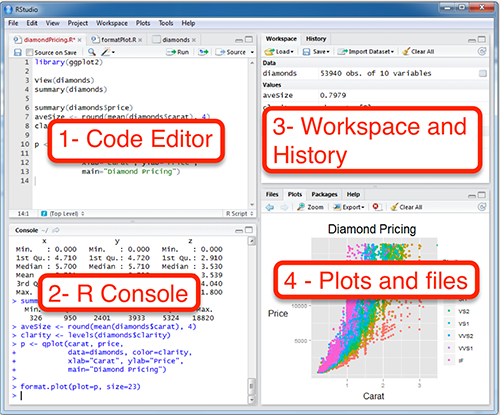
\includegraphics[width=0.5\linewidth]{fig/Rstudio} \end{figure}
\end{itemize}
\end{frame}

\begin{frame}{Typical Rstudio session}
\phantomsection\label{typical-rstudio-session-1}
\begin{itemize}
\tightlist
\item
  \textbf{Console}: output \& temporary input - usually unsaved

  \begin{figure}
  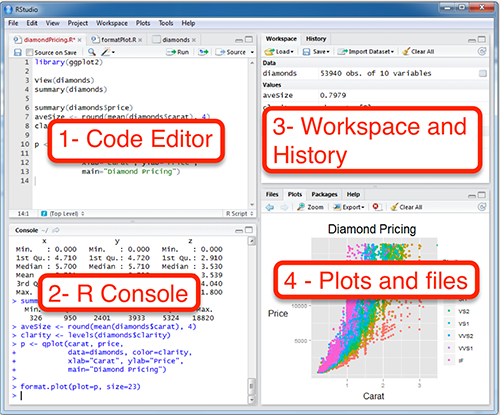
\includegraphics[width=0.5\linewidth]{fig/Rstudio} \end{figure}
\end{itemize}
\end{frame}

\begin{frame}{Typical Rstudio session}
\phantomsection\label{typical-rstudio-session-2}
\begin{itemize}
\tightlist
\item
  \textbf{Workspace}: Stores objects created during the session. Save
  with save.image().
\item
  \textbf{History}: Records commands used. Save with savehistory().
\end{itemize}

\begin{figure}
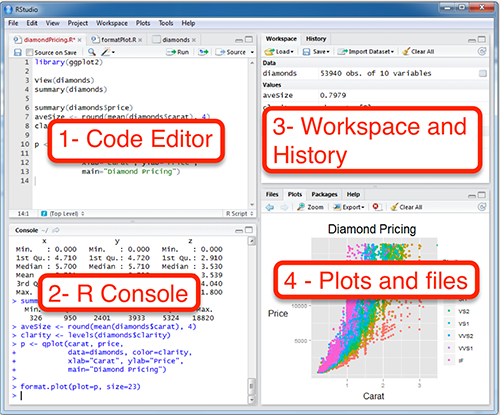
\includegraphics[width=0.5\linewidth]{fig/Rstudio} \end{figure}
\end{frame}

\begin{frame}{Typical Rstudio session}
\phantomsection\label{typical-rstudio-session-3}
\begin{itemize}
\tightlist
\item
  \textbf{Plots}: Displays graphs. Save plots with ggsave().
\item
  \textbf{Files}: Shows files in the working directory.
\end{itemize}

\begin{figure}
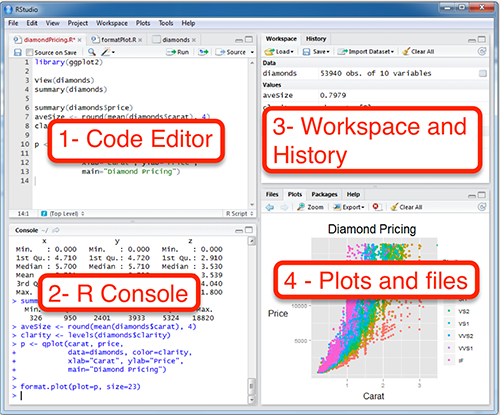
\includegraphics[width=0.5\linewidth]{fig/Rstudio} \end{figure}
\end{frame}

\begin{frame}{Data structures}
\phantomsection\label{data-structures}
\end{frame}

\begin{frame}{Data structures}
\phantomsection\label{data-structures-1}
\begin{itemize}
\tightlist
\item
  R is an object oriented programming language where an \textbf{object}
  is a generic term to describe something in R.
\end{itemize}

\begin{itemize}
\tightlist
\item
  There are many types of R-objects.\\
  Vectors\\
  Factors\\
  Lists\\
  Matrices\\
  Data Frames
\end{itemize}
\end{frame}

\begin{frame}[fragile]{Vectors in R}
\phantomsection\label{vectors-in-r}
\begin{itemize}
\tightlist
\item
  Vector is a sequence of elements of the same type (numeric, character,
  logical).
\end{itemize}

\begin{Shaded}
\begin{Highlighting}[]
\NormalTok{a }\OtherTok{\textless{}{-}} \FunctionTok{c}\NormalTok{(}\DecValTok{1}\NormalTok{,}\DecValTok{2}\NormalTok{,}\DecValTok{3}\NormalTok{,}\DecValTok{4}\NormalTok{,}\DecValTok{5}\NormalTok{)}
\NormalTok{b }\OtherTok{\textless{}{-}} \FunctionTok{c}\NormalTok{(}\DecValTok{6}\NormalTok{,}\DecValTok{7}\NormalTok{,}\DecValTok{8}\NormalTok{,}\DecValTok{9}\NormalTok{,}\DecValTok{10}\NormalTok{)}
\end{Highlighting}
\end{Shaded}

\begin{itemize}
\tightlist
\item
  Command \emph{c} creates a vector that is assigned to object a and b
\end{itemize}
\end{frame}

\begin{frame}[fragile]{Vectors in R}
\phantomsection\label{vectors-in-r-1}
\begin{itemize}
\tightlist
\item
  Two vectors of the same lenght can be addedd (a+a), multiply (a*a)
\end{itemize}

\begin{Shaded}
\begin{Highlighting}[]
\NormalTok{c }\OtherTok{\textless{}{-}}\NormalTok{ (a}\SpecialCharTok{+}\NormalTok{b)}
\NormalTok{c}
\end{Highlighting}
\end{Shaded}

\begin{verbatim}
## [1]  7  9 11 13 15
\end{verbatim}

\begin{Shaded}
\begin{Highlighting}[]
\NormalTok{d }\OtherTok{\textless{}{-}}\NormalTok{ (a}\SpecialCharTok{*}\NormalTok{b)}
\NormalTok{d}
\end{Highlighting}
\end{Shaded}

\begin{verbatim}
## [1]  6 14 24 36 50
\end{verbatim}
\end{frame}

\begin{frame}[fragile]{Vectors in R}
\phantomsection\label{vectors-in-r-2}
\begin{itemize}
\tightlist
\item
  Element in a vector can be sorter (\emph{sort()})
\end{itemize}

\begin{Shaded}
\begin{Highlighting}[]
\NormalTok{e }\OtherTok{\textless{}{-}} \FunctionTok{c}\NormalTok{(}\DecValTok{3}\NormalTok{,}\DecValTok{2}\NormalTok{,}\DecValTok{20}\NormalTok{,}\DecValTok{25}\NormalTok{,}\DecValTok{5}\NormalTok{)}
\FunctionTok{sort}\NormalTok{(e)}
\end{Highlighting}
\end{Shaded}

\begin{verbatim}
## [1]  2  3  5 20 25
\end{verbatim}
\end{frame}

\begin{frame}[fragile]{Factors in R}
\phantomsection\label{factors-in-r}
\begin{itemize}
\tightlist
\item
  Categorical data structure with predefined levels.
\end{itemize}

\begin{Shaded}
\begin{Highlighting}[]
\NormalTok{f }\OtherTok{\textless{}{-}} \FunctionTok{factor}\NormalTok{(}\FunctionTok{c}\NormalTok{(}\StringTok{"low"}\NormalTok{, }\StringTok{\textquotesingle{}medium\textquotesingle{}}\NormalTok{, }\StringTok{"high"}\NormalTok{, }\StringTok{\textquotesingle{}very high\textquotesingle{}}\NormalTok{))}
\end{Highlighting}
\end{Shaded}
\end{frame}

\begin{frame}{Data}
\phantomsection\label{data}
\begin{itemize}
\item
  R has three general classes for data:

  \begin{enumerate}
  \tightlist
  \item
    \textbf{list}: collection of objects of different lengths or classes
  \item
    \textbf{matrix}: vectors of the same length and same class
  \item
    \textbf{data.frame}: vectors of the same length and different
    classes
  \end{enumerate}
\end{itemize}
\end{frame}

\begin{frame}[fragile]{Lists}
\phantomsection\label{lists}
\begin{itemize}
\tightlist
\item
  A list is an R-object which can contain many different types of
  elements inside it like vectors, functions and even another list
  inside it.
\end{itemize}

\begin{Shaded}
\begin{Highlighting}[]
\CommentTok{\# Creating a list in R with various types of elements}
\NormalTok{my\_list }\OtherTok{\textless{}{-}} \FunctionTok{list}\NormalTok{(}
  \CommentTok{\# A numeric vector}
  \AttributeTok{Numbers =} \FunctionTok{c}\NormalTok{(}\DecValTok{1}\NormalTok{, }\DecValTok{2}\NormalTok{, }\DecValTok{3}\NormalTok{, }\DecValTok{4}\NormalTok{, }\DecValTok{5}\NormalTok{),}
  \CommentTok{\# A character vector}
  \AttributeTok{Words =} \FunctionTok{c}\NormalTok{(}\StringTok{"apple"}\NormalTok{, }\StringTok{"banana"}\NormalTok{, }\StringTok{"cherry"}\NormalTok{))}
\end{Highlighting}
\end{Shaded}
\end{frame}

\begin{frame}[fragile]{Lists}
\phantomsection\label{lists-1}
\begin{itemize}
\tightlist
\item
  A list is an R-object which can contain many different types of
  elements inside it like vectors, functions and even another list
  inside it.
\end{itemize}

\begin{Shaded}
\begin{Highlighting}[]
\NormalTok{  NestedList }\OtherTok{=} \FunctionTok{list}\NormalTok{(}
    \AttributeTok{Logical =} \FunctionTok{c}\NormalTok{(}\ConstantTok{TRUE}\NormalTok{, }\ConstantTok{FALSE}\NormalTok{, }\ConstantTok{TRUE}\NormalTok{),}
    \AttributeTok{Mixed =} \FunctionTok{c}\NormalTok{(}\FloatTok{3.14}\NormalTok{, }\StringTok{"pi"}\NormalTok{, }\ConstantTok{FALSE}\NormalTok{))}
\NormalTok{NestedList}
\end{Highlighting}
\end{Shaded}

\begin{verbatim}
## $Logical
## [1]  TRUE FALSE  TRUE
## 
## $Mixed
## [1] "3.14"  "pi"    "FALSE"
\end{verbatim}
\end{frame}

\begin{frame}[fragile]{Matrices}
\phantomsection\label{matrices}
\begin{itemize}
\tightlist
\item
  A matrix is a two-dimensional rectangular data set.
\item
  It can be created using a vector input to the matrix function.
\end{itemize}

\begin{Shaded}
\begin{Highlighting}[]
\CommentTok{\# Create a 3x3 matrix in R}
\NormalTok{my\_matrix }\OtherTok{\textless{}{-}} \FunctionTok{matrix}\NormalTok{(}
  \AttributeTok{data =} \DecValTok{1}\SpecialCharTok{:}\DecValTok{9}\NormalTok{,       }\CommentTok{\# Data to fill the matrix}
  \AttributeTok{nrow =} \DecValTok{3}\NormalTok{,         }\CommentTok{\# Number of rows}
  \AttributeTok{ncol =} \DecValTok{3}\NormalTok{,         }\CommentTok{\# Number of columns}
  \AttributeTok{byrow =} \ConstantTok{TRUE}\NormalTok{)      }\CommentTok{\# Fill the matrix by rows}
\NormalTok{my\_matrix}
\end{Highlighting}
\end{Shaded}

\begin{verbatim}
##      [,1] [,2] [,3]
## [1,]    1    2    3
## [2,]    4    5    6
## [3,]    7    8    9
\end{verbatim}
\end{frame}

\begin{frame}{Data Frames}
\phantomsection\label{data-frames}
\begin{itemize}
\tightlist
\item
  Data frames are tabular data objects.
\item
  \textbf{Unlike a matrix in data frame each column can contain
  different modes of data.}
\end{itemize}

\begin{itemize}
\tightlist
\item
  The first column can be numeric while the second column can be
  character and third column - Can be logical.
\end{itemize}

\begin{itemize}
\tightlist
\item
  It is a list of vectors of equal length.
\end{itemize}

\begin{itemize}
\tightlist
\item
  Data Frames are created using the \textbf{\emph{data.frame()}}
  function.
\end{itemize}

\begin{itemize}
\tightlist
\item
  When we execute the above code, it produces the following result:
\end{itemize}
\end{frame}

\begin{frame}{Table}
\phantomsection\label{table}
\begin{itemize}
\tightlist
\item
  Summary

  \begin{figure}
  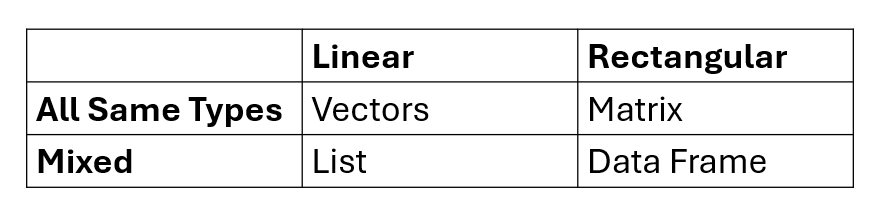
\includegraphics[width=0.8\linewidth]{fig/table} \end{figure}
\end{itemize}
\end{frame}

\begin{frame}{Reading data}
\phantomsection\label{reading-data}
\end{frame}

\begin{frame}[fragile]{Reading data}
\phantomsection\label{reading-data-1}
\begin{itemize}
\tightlist
\item
  Command for reading in text files is:
\end{itemize}

\begin{Shaded}
\begin{Highlighting}[]
\FunctionTok{read.table}\NormalTok{(}\StringTok{"suomi.txt"}\NormalTok{, }\AttributeTok{header=}\NormalTok{T, }\AttributeTok{sep=}\StringTok{"}\SpecialCharTok{\textbackslash{}t}\StringTok{"}\NormalTok{)}
\end{Highlighting}
\end{Shaded}

\begin{itemize}
\tightlist
\item
  This examples has one command with three arguments:

  \begin{itemize}
  \tightlist
  \item
    file name (in quotes)
  \item
    header that tells whether columns have titles
  \item
    sep that tells that the file is tab-delimited.
  \end{itemize}
\end{itemize}
\end{frame}

\begin{frame}[fragile]{Reading data}
\phantomsection\label{reading-data-2}
\begin{itemize}
\tightlist
\item
  \textbf{CSV File}
\item
  Usage: Reads comma-separated values, often used for structured data.
\end{itemize}

\begin{Shaded}
\begin{Highlighting}[]
\NormalTok{data }\OtherTok{\textless{}{-}} \FunctionTok{read.csv}\NormalTok{(}\StringTok{"file.csv"}\NormalTok{)}
\end{Highlighting}
\end{Shaded}

\begin{itemize}
\tightlist
\item
  \textbf{Text File}\\
\item
  Usage: Reads tabular data from a text file; sep can be adjusted for
  different delimiters.
\end{itemize}

\begin{Shaded}
\begin{Highlighting}[]
\NormalTok{data }\OtherTok{\textless{}{-}} \FunctionTok{read.table}\NormalTok{(}\StringTok{"file.txt"}\NormalTok{, }\AttributeTok{header =} \ConstantTok{TRUE}\NormalTok{, }\AttributeTok{sep =} \StringTok{"}\SpecialCharTok{\textbackslash{}t}\StringTok{"}\NormalTok{)}
\end{Highlighting}
\end{Shaded}

\begin{itemize}
\tightlist
\item
  \textbf{Excel File}
\item
  Usage: Reads data from Excel files; you can specify the sheet number
  or name.
\end{itemize}

\begin{Shaded}
\begin{Highlighting}[]
\FunctionTok{library}\NormalTok{(readxl)}
\NormalTok{data }\OtherTok{\textless{}{-}} \FunctionTok{read\_excel}\NormalTok{(}\StringTok{"file.xlsx"}\NormalTok{, }\AttributeTok{sheet =} \DecValTok{1}\NormalTok{)}
\end{Highlighting}
\end{Shaded}
\end{frame}

\begin{frame}[fragile]{Reading data}
\phantomsection\label{reading-data-3}
\begin{itemize}
\tightlist
\item
  Print the current working directory
\end{itemize}

\begin{Shaded}
\begin{Highlighting}[]
\FunctionTok{getwd}\NormalTok{()}
\end{Highlighting}
\end{Shaded}

\begin{itemize}
\tightlist
\item
  Change to my directory
\end{itemize}

\begin{Shaded}
\begin{Highlighting}[]
\FunctionTok{setwd}\NormalTok{(mydirectory)}
\FunctionTok{setwd}\NormalTok{(}\StringTok{"c:/docs/mydir"}\NormalTok{) }
\end{Highlighting}
\end{Shaded}
\end{frame}

\begin{frame}{Reading data}
\phantomsection\label{reading-data-4}
\begin{itemize}
\tightlist
\item
  Subscripts are given inside square brackets after the object's name:
\item
  df{[},1{]}

  \begin{itemize}
  \tightlist
  \item
    Gets the \textbf{first column} from the object dat
  \end{itemize}
\item
  df{[},1{]}

  \begin{itemize}
  \tightlist
  \item
    Gets the \textbf{first row} from the object dat
  \end{itemize}
\item
  df{[}1,1{]}

  \begin{itemize}
  \tightlist
  \item
    Gets the \textbf{first row} and it's \textbf{first column} from the
    object dat
  \end{itemize}
\end{itemize}
\end{frame}

\begin{frame}{Reading data}
\phantomsection\label{reading-data-5}
\begin{itemize}
\tightlist
\item
  Subscripts can be used for, e.g., extracting a subset of the data:

  \begin{itemize}
  \tightlist
  \item
    df{[}which(df\$year\textgreater1900),{]}

    \begin{itemize}
    \item
      Now, this takes a bit of pondering to work out.
    \item
      First we have the object df, and we are accessing a part of it,
      because it's name is followed by the square brackets
    \item
      Then we have one command (which) that makes an evaluation whether
      the column year in the object df has a value higher than 1900.
    \item
      Last the subscript ends with a comma, that tells us that we are
      accessing rows.
    \item
      So this command takes all the rows that have a year higher 1900
      from the object dat that is a data frame.
    \end{itemize}
  \end{itemize}
\end{itemize}
\end{frame}

\begin{frame}{Assigning Values in R}
\phantomsection\label{assigning-values-in-r}
\begin{itemize}
\tightlist
\item
  In R, you can assign values to objects using the syntax object
  \textless- value
\item
  An arrow (\textless-) formed by a smaller than character and a hyphen
  without a space!
\item
  The equal character (=).
\end{itemize}
\end{frame}

\begin{frame}{R Warning!}
\phantomsection\label{r-warning}
\begin{itemize}
\tightlist
\item
  Naming objects:

  \begin{itemize}
  \tightlist
  \item
    R is a case sensitive language.
  \item
    FOO, Foo, and foo are three different objects
  \item
    Object names can't start with a number
  \item
    Never use special characters, such as å, ä, or ö in object names.
  \end{itemize}
\end{itemize}
\end{frame}

\begin{frame}{Using Functions in R}
\phantomsection\label{using-functions-in-r}
\begin{itemize}
\tightlist
\item
  R is a function based language where a \textbf{\emph{function}} takes
  in some input and produces some output.

  \begin{itemize}
  \tightlist
  \item
    Vegas rules: what happens in a function, stays in a function.
  \end{itemize}
\end{itemize}
\end{frame}

\begin{frame}[fragile]{Data Visualization in R}
\phantomsection\label{data-visualization-in-r}
\begin{itemize}
\tightlist
\item
  Most powerful approach to statistical graphs, based on the
  \textbf{Grammar of Graphics}.
\end{itemize}

\begin{itemize}
\tightlist
\item
  A graphics language, composed of layers, \textbf{geoms} (points,
  lines, regions), each with graphical \textbf{aesthetics} (color, size,
  shape)
\end{itemize}

\begin{Shaded}
\begin{Highlighting}[]
\FunctionTok{library}\NormalTok{(ggplot2)}
\end{Highlighting}
\end{Shaded}

\begin{verbatim}
## Warning: package 'ggplot2' was built under R version 4.3.3
\end{verbatim}

\begin{Shaded}
\begin{Highlighting}[]
\FunctionTok{library}\NormalTok{(palmerpenguins)}
\end{Highlighting}
\end{Shaded}

\begin{verbatim}
## Warning: package 'palmerpenguins' was built under R version 4.3.2
\end{verbatim}
\end{frame}

\begin{frame}[fragile]{An Introduction to ggplot2}
\phantomsection\label{an-introduction-to-ggplot2}
\begin{Shaded}
\begin{Highlighting}[]
\FunctionTok{ggplot}\NormalTok{(}\AttributeTok{data =}\NormalTok{ penguins, }\FunctionTok{aes}\NormalTok{(}\AttributeTok{x =}\NormalTok{ flipper\_length\_mm, }
                          \AttributeTok{y =}\NormalTok{ body\_mass\_g)) }\SpecialCharTok{+}
    \FunctionTok{geom\_point}\NormalTok{(}\FunctionTok{aes}\NormalTok{(}\AttributeTok{color =}\NormalTok{ species, }\AttributeTok{shape =}\NormalTok{ species))}
\end{Highlighting}
\end{Shaded}

\begin{verbatim}
## Warning: Removed 2 rows containing missing values or values outside the scale range
## (`geom_point()`).
\end{verbatim}

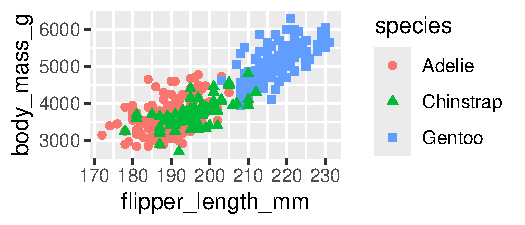
\includegraphics{M3-R-Basics_files/figure-beamer/unnamed-chunk-21-1.pdf}
\end{frame}

\begin{frame}[fragile]{An Introduction to ggplot2}
\phantomsection\label{an-introduction-to-ggplot2-1}
\begin{Shaded}
\begin{Highlighting}[]
\FunctionTok{ggplot}\NormalTok{(}\AttributeTok{data =} \SpecialCharTok{\textless{}}\NormalTok{your data set}\SpecialCharTok{\textgreater{}}\NormalTok{, }\FunctionTok{aes}\NormalTok{(}\AttributeTok{x =} \SpecialCharTok{\textless{}}\NormalTok{x axis variable}\SpecialCharTok{\textgreater{}}\NormalTok{, }
                                   \AttributeTok{y =} \SpecialCharTok{\textless{}}\NormalTok{y axis variable}\SpecialCharTok{\textgreater{}}\NormalTok{)) }\SpecialCharTok{+}
    \FunctionTok{geom\_point}\NormalTok{(}\FunctionTok{aes}\NormalTok{(}\AttributeTok{size =} \SpecialCharTok{\textless{}}\NormalTok{size variable}\SpecialCharTok{\textgreater{}}\NormalTok{, }
                   \AttributeTok{color =} \SpecialCharTok{\textless{}}\NormalTok{color variable}\SpecialCharTok{\textgreater{}}\NormalTok{, }
                   \AttributeTok{shape =} \SpecialCharTok{\textless{}}\NormalTok{shape variable}\SpecialCharTok{\textgreater{}}\NormalTok{))}
\end{Highlighting}
\end{Shaded}
\end{frame}

\end{document}
